\section{遮挡}
在光栅化时,有一个重要的问题是我们如何判断前后遮挡关系。朴素的解决方案是,我们谨慎的从后到前的渲染图形,这样靠前的图形会自然覆盖掉靠后的图形。然而,,找到一个正确的从后到前的渲染顺序是非常麻烦的,且有些情况下,我们不可能找到这样的顺序,例如
\begin{itemize}
    \item 设想$A,B$两个三角面,$A$和$B$的三角面在三维空间中相交。
    \item 设想$A,B,C$三个三角面,$A$部分遮挡$B$,$B$部分遮挡$C$,$C$部分遮挡$A$。
\end{itemize}

\begin{Figure}[三角面的相互遮挡]
    \begin{FigureSub}[两个三角面相互穿过]
        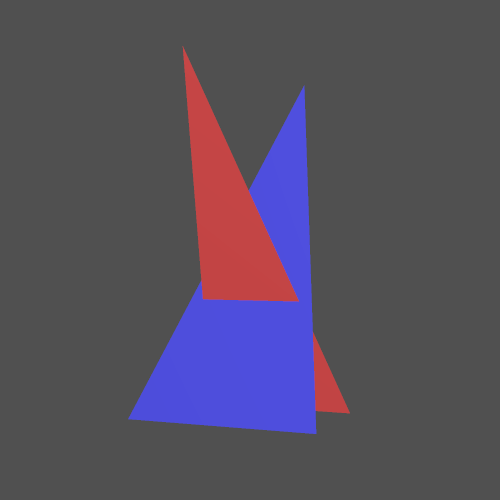
\includegraphics[width=6.5cm]{image/RasterizationIOW/TrianglesA.png}
    \end{FigureSub}
    \hspace{0.5cm}
    \begin{FigureSub}[三个三角面循环遮挡]
        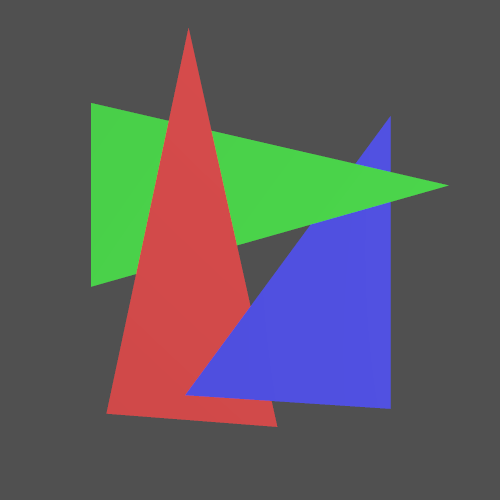
\includegraphics[width=6.5cm]{image/RasterizationIOW/TrianglesB.png}
    \end{FigureSub}
\end{Figure}

通过$z$-buffer可以更简单的解决该问题,它为每个像素在RGB颜色外增加了一个$z$分量,它代表该像素目前为止来自多近的物体。当光栅化一个三角面时,我们可以通过和RGB颜色一样的方法,通过三角面顶点处的$z$值插值出每个像素出的$z$值。随后,我们会就该三角面每个像素的$z$值与$z$-buffer中存储的值进行比较。若当前的$z$值更大,则说明之前已经有比当前三角面更近的三角面绘制了该像素,换言之,当前三角面在该像素位置是被遮挡的,应当跳过这一像素的绘制。若当前的$z$值更小,应当覆盖绘制这一像素并更新$z$-buffer中的存储值。

\xref{fig:$z$-buffer的效果}展示了$z$-buffer的实际效果,将其用一张灰度图可视化,越亮代表与相机距离越近。

\begin{Figure}[$z$-buffer的效果]
    \begin{FigureSub}[渲染图像]
        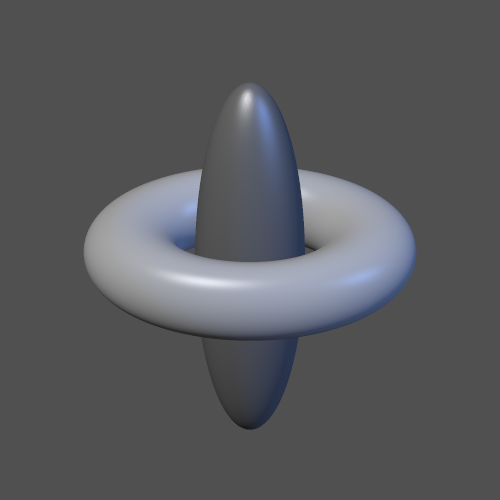
\includegraphics[width=6.5cm]{image/RasterizationIOW/SphereRing.png}
    \end{FigureSub}\\
    \vspace{0.5cm}
    \begin{FigureSub}[渲染图像的$z$-buffer]
        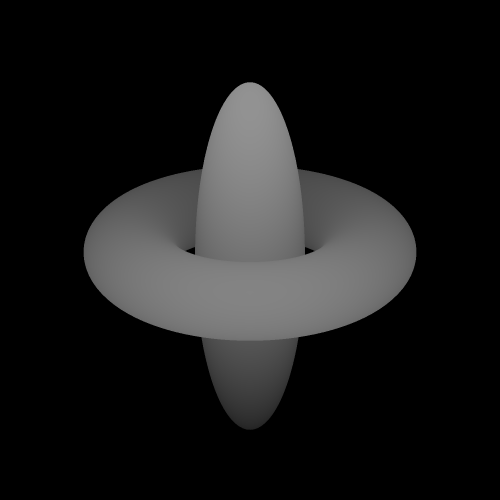
\includegraphics[width=6.5cm]{image/RasterizationIOW/SphereRingZbuff.png}
    \end{FigureSub}
\end{Figure}

这里有一个问题,由于$z$是和RGB颜色一并处理的,我们通常会用整数而不是浮点数来存储$z$值。这可能造成精度问题,我们需要判断什么情况下该问题不会影响前后关系的判断。

在\xref{sec:透视投影变换}中,我们知道透视变换对$z$的变换是\setpeq{遮挡的精度问题}
\begin{Equation}&[1]
    z'=z_n+z_f-\frac{z_nz_f}{z}
\end{Equation}
我们求$z'$相对$z$的微分,并以之近似差分
\begin{Equation}&[2]
    \delt{z}'=\frac{z_nz_f\delt{z}}{z}
\end{Equation}
请注意,光栅化阶段中,在$z$-buffer内存储的$z$值和三角面顶点记录的$z$值实际上是变换后的$z'$的值,假如我们使用$b$位的二进制数来存储$z'$值,那最小允许的$\delt{z}'$的间隔应是
\begin{Equation}&[3]
    \delt{z}'=\frac{z_f-z_n}{2^b}
\end{Equation}

结合\xrefpeq{2}和\xrefpeq{3}可以得到
\begin{Equation}
    \delt{z}=\frac{z(z_f-z_n)}{z_nz_f 2^b}
\end{Equation}
这表明在实际空间中不同深度$z$处允许的最小间隔$\delt{z}$是不等的,考虑到$z$至$z'$的非线性变换关系,这是合理的。最糟的情况出现在$z=z_f$时,此时最小允许间隔是最大的
\begin{Equation}
    \delt{z}=\frac{z_f-z_n}{z_n 2^b}
\end{Equation}
整理如下
\begin{BoxFormula}[深度的精度问题]
    若使用$b$位二进制量化深度,则实际空间的深度间隔不得低于该值
    \begin{Equation}
        \delt{z}=\frac{z_f-z_n}{z_n 2^b}
    \end{Equation}
\end{BoxFormula}
